\documentclass[11pt,a4paper]{article}
\usepackage[utf8]{inputenc}
\usepackage[T1]{fontenc}
\usepackage{amsmath,amssymb,amsthm}
\usepackage{tikz}
\usetikzlibrary{shapes,arrows,positioning,calc,decorations.pathreplacing,patterns,arrows.meta}
\usepackage{pgfplots}
\pgfplotsset{compat=1.17}
\usepackage{geometry}
\geometry{margin=1in}
\usepackage{booktabs}
\usepackage{xcolor}
\usepackage{tcolorbox}
\usepackage{float}

\definecolor{fepblue}{RGB}{41,128,185}
\definecolor{crrgreen}{RGB}{39,174,96}
\definecolor{goalred}{RGB}{192,57,43}
\definecolor{matchpurple}{RGB}{142,68,173}

\tcbuselibrary{theorems,skins}

\newtcbtheorem[number within=section]{fepbox}{FEP Formulation}{
  colback=fepblue!10,
  colframe=fepblue,
  fonttitle=\bfseries
}{fep}

\newtcbtheorem[number within=section]{crrbox}{CRR Formulation}{
  colback=crrgreen!10,
  colframe=crrgreen,
  fonttitle=\bfseries
}{crr}

\newtcbtheorem[number within=section]{matchbox}{Inside-Outside Match}{
  colback=matchpurple!10,
  colframe=matchpurple,
  fonttitle=\bfseries
}{match}

\title{\textbf{The Journey from A to B:}\\[0.5em]
\Large A Mathematical Analysis of Goal-Directed Behavior\\Through Free Energy Principle and CRR Frameworks}
\author{CRR Research Analysis}
\date{January 2026}

\begin{document}

\maketitle

\begin{abstract}
We present a detailed mathematical analysis of a complete driving journey from location A to location B, expressed simultaneously in the Free Energy Principle (FEP) / Active Inference framework and the Coherence-Rupture-Regeneration (CRR) framework. We demonstrate that CRR provides the \emph{dynamical grammar} specifying \emph{when} and \emph{how} the belief updates of active inference occur. The journey is decomposed into nested hierarchical goals, each exhibiting the characteristic pattern: coherence accumulation toward a goal state (prediction), rupture when inside matches outside (prediction confirmation/violation), and regeneration that either reinforces or rewires the agent's model. We show that the universal threshold $\Omega \approx 16$ nats represents the information capacity required to specify a goal with sufficient precision for successful action.
\end{abstract}

\tableofcontents
\newpage

%=============================================================================
\section{Introduction: Two Frameworks, One Process}
%=============================================================================

Consider the seemingly simple act of driving from your home (A) to your workplace (B). This journey involves hundreds of nested decisions, predictions, actions, and updates---from the macro-level navigation to micro-level muscle contractions. We analyze this through two complementary mathematical frameworks:

\begin{itemize}
    \item \textbf{Free Energy Principle (FEP)}: The brain minimizes variational free energy, which bounds surprise. Action and perception work together to bring predictions and observations into alignment.
    \item \textbf{Coherence-Rupture-Regeneration (CRR)}: Information coherence accumulates until reaching a threshold $\Omega$, triggering rupture and subsequent regeneration that updates the system's state.
\end{itemize}

\begin{matchbox}{The Central Insight}{}
The CRR framework provides the \textbf{dynamical grammar} of active inference---it specifies:
\begin{enumerate}
    \item \textbf{When} belief updates occur (at rupture, when $C = \Omega$)
    \item \textbf{How much} historical context influences the update (via $\exp(C/\Omega)$ weighting)
    \item \textbf{What form} the update takes (regeneration as Bayesian posterior update)
\end{enumerate}
The ``inside-outside match'' occurs precisely at rupture: the moment when accumulated evidence ($C$) reaches the precision of the goal specification ($\Omega$).
\end{matchbox}

%=============================================================================
\section{Mathematical Foundations}
%=============================================================================

\subsection{The Free Energy Principle}

Under the FEP, an agent maintains a generative model $p(o, s)$ of observations $o$ given hidden states $s$. The agent approximates the true posterior $p(s|o)$ with a recognition density $q(s)$.

\begin{fepbox}{Variational Free Energy}{}
\begin{equation}
F = \underbrace{\mathbb{E}_{q}[\ln q(s) - \ln p(s)]}_{\text{Complexity}} - \underbrace{\mathbb{E}_{q}[\ln p(o|s)]}_{\text{Accuracy}}
\end{equation}
Equivalently:
\begin{equation}
F = D_{KL}[q(s) \| p(s|o)] - \ln p(o) \geq -\ln p(o) = \text{Surprise}
\end{equation}
\end{fepbox}

The agent minimizes $F$ through:
\begin{itemize}
    \item \textbf{Perception}: Update $q(s)$ to better match observations
    \item \textbf{Action}: Change observations $o$ to match predictions
\end{itemize}

For active inference with goals, we introduce preferences $p(o|\mathcal{G})$ where $\mathcal{G}$ represents the goal:

\begin{fepbox}{Expected Free Energy (Goal-Directed)}{}
\begin{equation}
G(\pi) = \underbrace{\mathbb{E}_{\tilde{q}}[D_{KL}[q(s|\pi) \| q(s|o,\pi)]]}_{\text{Epistemic value (information gain)}} + \underbrace{\mathbb{E}_{\tilde{q}}[D_{KL}[q(o|\pi) \| p(o|\mathcal{G})]]}_{\text{Pragmatic value (goal achievement)}}
\end{equation}
where $\pi$ is a policy (sequence of actions) and $\tilde{q}$ is the predictive distribution.
\end{fepbox}

\subsection{The CRR Framework}

The CRR framework describes how systems accumulate coherent information until a phase transition.

\begin{crrbox}{Core Definitions}{}
\textbf{Coherence} accumulates evidence toward a goal:
\begin{equation}
C(t) = \int_0^t L(x(\tau), \tau) \, d\tau
\end{equation}
where $L$ is the coherence density (related to log-likelihood or prediction confirmation).

\textbf{Rupture} occurs when coherence reaches threshold:
\begin{equation}
\text{Rupture at } t^* \text{ when } C(t^*) = \Omega
\end{equation}

\textbf{Regeneration} updates the system state:
\begin{equation}
R[\phi](t) = \int_{-\infty}^{t} \phi(\tau) \cdot \exp\left(\frac{C(\tau)}{\Omega}\right) \cdot \Theta(t - \tau) \, d\tau
\end{equation}
\end{crrbox}

\subsection{The Correspondence}

We now establish the mathematical correspondence between frameworks:

\begin{table}[H]
\centering
\begin{tabular}{@{}lll@{}}
\toprule
\textbf{Concept} & \textbf{FEP/Active Inference} & \textbf{CRR} \\
\midrule
Goal state & Prior preference $p(o|\mathcal{G})$ & Threshold $\Omega$ \\
Evidence accumulation & $-\ln p(o|s)$ integration & Coherence $C(t)$ \\
Prediction error & $\varepsilon = o - g(\mu)$ & $dC/dt = L(x,t)$ \\
Inside-outside match & $F \to F_{\min}$ & $C \to \Omega$ \\
Belief update & Posterior $q(s|o)$ & Regeneration $R[\phi]$ \\
Precision weighting & $\Pi = \partial^2 F/\partial \mu^2$ & $\exp(C/\Omega)$ \\
\bottomrule
\end{tabular}
\caption{Mathematical correspondence between FEP and CRR frameworks}
\end{table}

\begin{matchbox}{The Key Equation}{}
At rupture ($C = \Omega$), the CRR regeneration weight equals Euler's number:
\begin{equation}
\exp\left(\frac{C}{\Omega}\right)\bigg|_{C=\Omega} = e \approx 2.718
\end{equation}
This corresponds to the FEP condition where free energy reaches its minimum for the current goal:
\begin{equation}
\frac{\partial F}{\partial q} = 0 \quad \Leftrightarrow \quad q(s) = p(s|o)
\end{equation}
The ``$e$-fold'' weighting represents optimal Bayesian integration of historical evidence.
\end{matchbox}

%=============================================================================
\section{The Driving Journey: Hierarchical Goal Structure}
%=============================================================================

\begin{figure}[H]
\centering
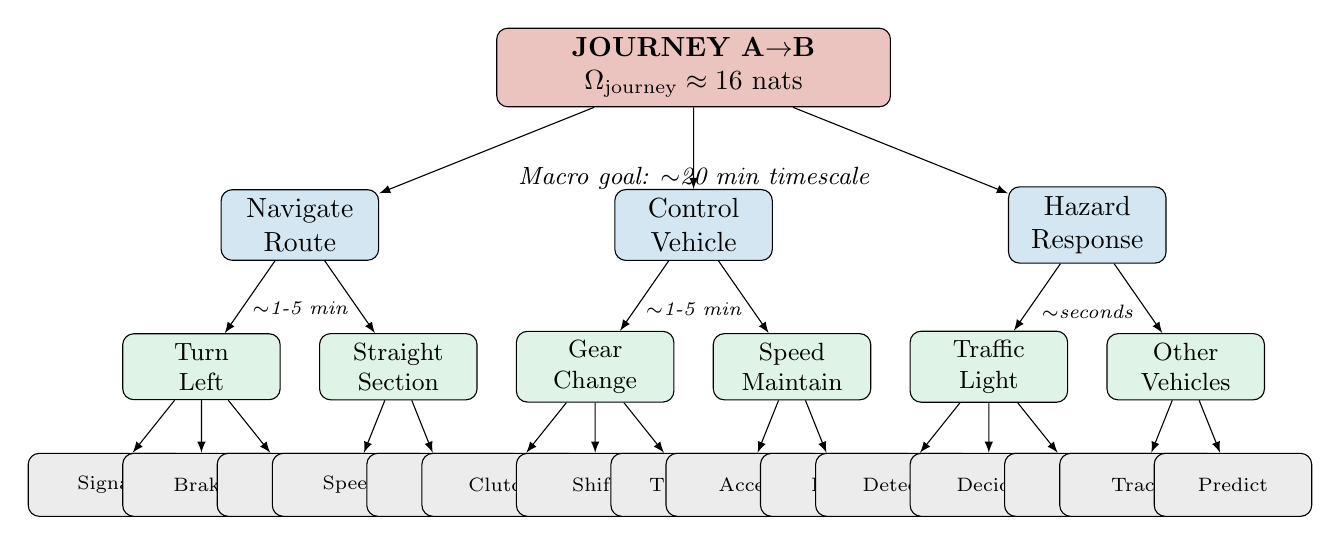
\begin{tikzpicture}[
    level 1/.style={sibling distance=50mm, level distance=20mm},
    level 2/.style={sibling distance=25mm, level distance=18mm},
    level 3/.style={sibling distance=12mm, level distance=15mm},
    every node/.style={draw, rounded corners, align=center, minimum width=20mm, minimum height=8mm},
    edge from parent/.style={draw, -latex}
]
\node[fill=goalred!30, minimum width=50mm] (root) {\textbf{JOURNEY A$\to$B}\\$\Omega_{\text{journey}} \approx 16$ nats}
    child {node[fill=fepblue!20] (nav) {Navigate\\Route}
        child {node[fill=crrgreen!15, font=\small] {Turn\\Left}
            child {node[fill=gray!15, font=\scriptsize] {Signal}}
            child {node[fill=gray!15, font=\scriptsize] {Brake}}
            child {node[fill=gray!15, font=\scriptsize] {Steer}}
        }
        child {node[fill=crrgreen!15, font=\small] {Straight\\Section}
            child {node[fill=gray!15, font=\scriptsize] {Speed}}
            child {node[fill=gray!15, font=\scriptsize] {Lane}}
        }
    }
    child {node[fill=fepblue!20] (vehicle) {Control\\Vehicle}
        child {node[fill=crrgreen!15, font=\small] {Gear\\Change}
            child {node[fill=gray!15, font=\scriptsize] {Clutch}}
            child {node[fill=gray!15, font=\scriptsize] {Shift}}
            child {node[fill=gray!15, font=\scriptsize] {Throttle}}
        }
        child {node[fill=crrgreen!15, font=\small] {Speed\\Maintain}
            child {node[fill=gray!15, font=\scriptsize] {Accel}}
            child {node[fill=gray!15, font=\scriptsize] {Brake}}
        }
    }
    child {node[fill=fepblue!20] (hazard) {Hazard\\Response}
        child {node[fill=crrgreen!15, font=\small] {Traffic\\Light}
            child {node[fill=gray!15, font=\scriptsize] {Detect}}
            child {node[fill=gray!15, font=\scriptsize] {Decide}}
            child {node[fill=gray!15, font=\scriptsize] {Act}}
        }
        child {node[fill=crrgreen!15, font=\small] {Other\\Vehicles}
            child {node[fill=gray!15, font=\scriptsize] {Track}}
            child {node[fill=gray!15, font=\scriptsize] {Predict}}
        }
    };

\node[below=5mm of root, draw=none, font=\small\itshape] {Macro goal: $\sim$20 min timescale};
\node[below=2mm of nav, draw=none, font=\scriptsize\itshape, text width=25mm, align=center] {$\sim$1-5 min};
\node[below=2mm of vehicle, draw=none, font=\scriptsize\itshape, text width=25mm, align=center] {$\sim$1-5 min};
\node[below=2mm of hazard, draw=none, font=\scriptsize\itshape, text width=25mm, align=center] {$\sim$seconds};
\end{tikzpicture}
\caption{Hierarchical goal structure of a driving journey. Each level contains nested CRR cycles, all governed by the same $\Omega \approx 16$ nats threshold for ``inside-outside match.''}
\label{fig:hierarchy}
\end{figure}

%=============================================================================
\section{Detailed Analysis: Micro-Goals in FEP and CRR}
%=============================================================================

\subsection{Example 1: Gear Change}

Consider shifting from 2nd to 3rd gear as RPM approaches 3000.

\begin{figure}[H]
\centering
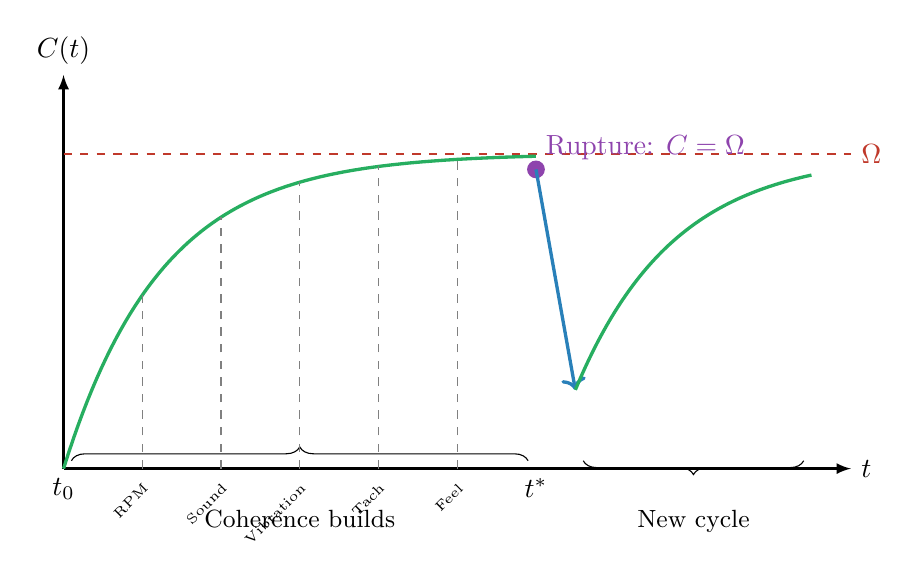
\begin{tikzpicture}[scale=1]
% Time axis
\draw[-latex, thick] (0,0) -- (10,0) node[right] {$t$};
\draw[-latex, thick] (0,0) -- (0,5) node[above] {$C(t)$};

% Omega threshold
\draw[dashed, thick, goalred] (0,4) -- (10,4) node[right] {$\Omega$};

% Coherence curve
\draw[very thick, crrgreen, domain=0:6, samples=100]
    plot (\x, {4*(1 - exp(-0.8*\x))});

% Rupture point
\filldraw[matchpurple] (6,3.8) circle (3pt);
\node[above right, matchpurple] at (6,3.8) {Rupture: $C = \Omega$};

% Regeneration
\draw[very thick, fepblue, ->] (6,3.8) -- (6.5,1);
\draw[very thick, crrgreen, domain=6.5:9.5, samples=100]
    plot (\x, {1 + 3*(1 - exp(-0.8*(\x-6.5)))});

% Labels
\node[below] at (0,0) {$t_0$};
\node[below] at (6,0) {$t^*$};

% Annotations
\draw[decorate, decoration={brace, amplitude=5pt}] (0.1,0.1) -- (5.9,0.1);
\node[below, font=\small] at (3,-0.4) {Coherence builds};

\draw[decorate, decoration={brace, amplitude=5pt, mirror}] (6.6,0.1) -- (9.4,0.1);
\node[below, font=\small] at (8,-0.4) {New cycle};

% Evidence markers
\foreach \x/\label in {1/RPM, 2/Sound, 3/Vibration, 4/Tach, 5/Feel} {
    \draw[gray, dashed] (\x,0) -- (\x,{4*(1 - exp(-0.8*\x))});
    \node[below, font=\tiny, rotate=45, anchor=north east] at (\x,0) {\label};
}
\end{tikzpicture}
\caption{CRR dynamics for a gear change. Coherence accumulates from multiple sensory channels until rupture triggers the shift action.}
\label{fig:gearchange}
\end{figure}

\begin{fepbox}{Gear Change in FEP Terms}{}
\textbf{Generative model}: $p(o, s) = p(\text{RPM}, \text{sound}, \text{vibration} | \text{gear}, \text{speed}) \cdot p(\text{gear}, \text{speed})$

\textbf{Goal preference}: $p(o|\mathcal{G}) = \mathcal{N}(\text{RPM}; 2000, \sigma^2)$ (prefer RPM around 2000)

\textbf{Free energy before shift} (RPM at 3000):
\begin{equation}
F_{\text{before}} = \frac{1}{2\sigma^2}(3000 - 2000)^2 + \text{const} = \frac{10^6}{2\sigma^2}
\end{equation}

\textbf{Expected free energy of shift policy} $\pi_{\text{shift}}$:
\begin{equation}
G(\pi_{\text{shift}}) = \mathbb{E}\left[\frac{1}{2\sigma^2}(\text{RPM}_{\text{after}} - 2000)^2\right] \approx \frac{(2100-2000)^2}{2\sigma^2} = \frac{10^4}{2\sigma^2}
\end{equation}

\textbf{Action selection}: $\pi^* = \arg\min_\pi G(\pi) = \pi_{\text{shift}}$ (shift minimizes expected free energy)
\end{fepbox}

\begin{crrbox}{Gear Change in CRR Terms}{}
\textbf{Coherence accumulation}:
\begin{equation}
C(t) = \int_0^t \left[ L_{\text{RPM}}(\tau) + L_{\text{sound}}(\tau) + L_{\text{vibration}}(\tau) + L_{\text{tach}}(\tau) \right] d\tau
\end{equation}

Each channel contributes $\sim 4-6$ bits to coherence:
\begin{itemize}
    \item $L_{\text{RPM}}$: Tachometer reading $\to$ 5 bits
    \item $L_{\text{sound}}$: Engine pitch $\to$ 4 bits
    \item $L_{\text{vibration}}$: Proprioceptive $\to$ 5 bits
    \item $L_{\text{feel}}$: Acceleration feel $\to$ 4 bits
\end{itemize}

\textbf{Total at rupture}: $C(t^*) = 18-20$ bits $\approx 13-14$ nats $\to \Omega$

\textbf{Rupture}: ``Now is the moment to shift'' -- inside (prediction of optimal shift point) matches outside (sensory evidence confirms)

\textbf{Regeneration}:
\begin{equation}
R[\phi_{\text{motor}}] = \int \phi_{\text{motor}}(\tau) \cdot e \cdot \Theta(t-\tau) \, d\tau
\end{equation}
Historical motor pattern (clutch-shift-throttle sequence) is weighted by $e$ and executed.
\end{crrbox}

\begin{matchbox}{The Inside-Outside Match for Gear Change}{}
\textbf{Inside} (prediction/goal): ``When RPM $\approx$ 3000, shift to maintain efficiency''

\textbf{Outside} (observation): Tachometer, engine sound, vibration all indicate RPM $\approx$ 3000

\textbf{Match condition}:
\begin{equation}
\underbrace{C(t^*)}_{\substack{\text{Accumulated}\\\text{evidence}}} = \underbrace{\Omega}_{\substack{\text{Goal}\\\text{precision}}} \quad \Leftrightarrow \quad \underbrace{F \to F_{\min}}_{\substack{\text{Free energy}\\\text{minimized}}}
\end{equation}

\textbf{Outcome branches}:
\begin{itemize}
    \item \textbf{Success} (smooth shift): Regeneration \emph{reinforces} motor program $\to$ lower $\Omega$ next time (more automatic)
    \item \textbf{Failure} (grind): Regeneration \emph{rewires} timing $\to$ adjust clutch-throttle coordination
\end{itemize}
\end{matchbox}

\subsection{Example 2: Traffic Light Response}

\begin{figure}[H]
\centering
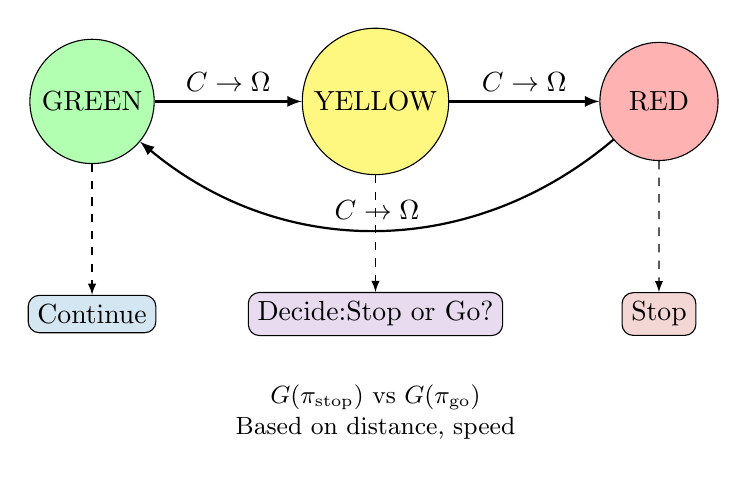
\begin{tikzpicture}[scale=0.9]
% State diagram
\node[draw, circle, fill=green!30, minimum size=15mm] (green) at (0,0) {GREEN};
\node[draw, circle, fill=yellow!50, minimum size=15mm] (yellow) at (4,0) {YELLOW};
\node[draw, circle, fill=red!30, minimum size=15mm] (red) at (8,0) {RED};

% Transitions
\draw[-latex, thick] (green) -- node[above] {$C \to \Omega$} (yellow);
\draw[-latex, thick] (yellow) -- node[above] {$C \to \Omega$} (red);
\draw[-latex, thick, bend left=40] (red) to node[above] {$C \to \Omega$} (green);

% Agent responses below
\node[draw, rounded corners, fill=fepblue!20] (cont) at (0,-3) {Continue};
\node[draw, rounded corners, fill=matchpurple!20] (decide) at (4,-3) {Decide:\\Stop or Go?};
\node[draw, rounded corners, fill=goalred!20] (stop) at (8,-3) {Stop};

\draw[-latex, dashed] (green) -- (cont);
\draw[-latex, dashed] (yellow) -- (decide);
\draw[-latex, dashed] (red) -- (stop);

% Decision detail
\node[below=5mm of decide, font=\small, text width=40mm, align=center] {
$G(\pi_{\text{stop}})$ vs $G(\pi_{\text{go}})$\\
Based on distance, speed
};
\end{tikzpicture}
\caption{Traffic light state transitions and corresponding agent decisions. Each state transition represents a CRR cycle with rupture triggering action selection.}
\end{figure}

\begin{fepbox}{Traffic Light in FEP: The Yellow Light Dilemma}{}
At yellow light onset, the agent must select between policies:

\textbf{Policy 1} ($\pi_{\text{stop}}$): Brake and stop before intersection
\begin{equation}
G(\pi_{\text{stop}}) = \underbrace{0}_{\text{epistemic}} + \underbrace{D_{KL}[q(o|\pi_{\text{stop}}) \| p(o|\mathcal{G}_{\text{safety}})]}_{\text{pragmatic: safety cost}}
\end{equation}

\textbf{Policy 2} ($\pi_{\text{go}}$): Accelerate through intersection
\begin{equation}
G(\pi_{\text{go}}) = \underbrace{H[p(o|\pi_{\text{go}})]}_{\text{epistemic: uncertainty}} + \underbrace{D_{KL}[q(o|\pi_{\text{go}}) \| p(o|\mathcal{G}_{\text{safety}})]}_{\text{pragmatic: risk if red}}
\end{equation}

\textbf{Decision boundary}: At distance $d^*$ and speed $v^*$:
\begin{equation}
G(\pi_{\text{stop}}) = G(\pi_{\text{go}}) \quad \Rightarrow \quad \text{``Point of no return''}
\end{equation}
\end{fepbox}

\begin{crrbox}{Traffic Light in CRR: Evidence Accumulation}{}
\textbf{Coherence channels}:
\begin{align}
L_{\text{visual}}(t) &= \text{Light color recognition} \approx 3 \text{ bits} \\
L_{\text{distance}}(t) &= \text{Distance to intersection} \approx 5 \text{ bits} \\
L_{\text{speed}}(t) &= \text{Current velocity} \approx 4 \text{ bits} \\
L_{\text{traffic}}(t) &= \text{Other vehicles} \approx 4 \text{ bits} \\
L_{\text{timing}}(t) &= \text{Yellow duration estimate} \approx 3 \text{ bits}
\end{align}

\textbf{Total coherence}: $C = 19-20$ bits $\approx 14$ nats

\textbf{Rupture condition}: When $C = \Omega \approx 16$ nats, decision crystallizes:
\begin{equation}
\text{Action} = \begin{cases}
\text{Brake} & \text{if } C_{\text{stop}} > C_{\text{go}} \\
\text{Accelerate} & \text{if } C_{\text{go}} > C_{\text{stop}}
\end{cases}
\end{equation}
\end{crrbox}

\subsection{Example 3: Lane Change Maneuver}

\begin{figure}[H]
\centering
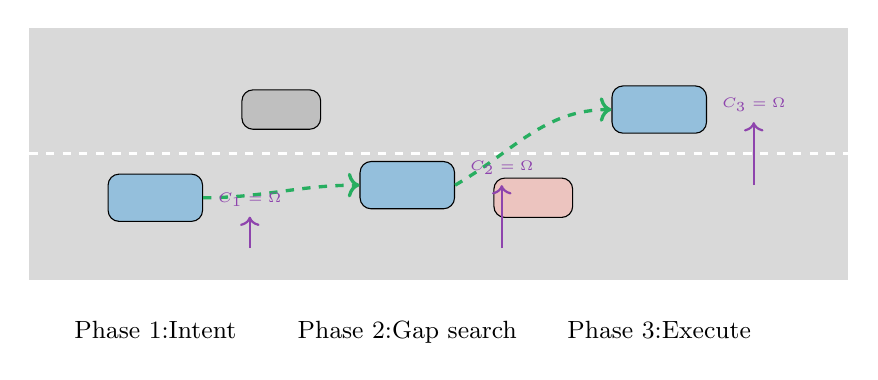
\begin{tikzpicture}[scale=0.8]
% Road
\fill[gray!30] (-1,-1) rectangle (12,3);
\draw[white, very thick, dashed] (-1,1) -- (12,1);

% Cars
\node[draw, fill=fepblue!50, minimum width=12mm, minimum height=6mm, rounded corners] (ego1) at (1,0.3) {};
\node[draw, fill=fepblue!50, minimum width=12mm, minimum height=6mm, rounded corners] (ego2) at (5,0.5) {};
\node[draw, fill=fepblue!50, minimum width=12mm, minimum height=6mm, rounded corners] (ego3) at (9,1.7) {};

% Trajectory
\draw[crrgreen, very thick, dashed, ->] (ego1.east) to[out=0, in=180] (ego2.west);
\draw[crrgreen, very thick, dashed, ->] (ego2.east) to[out=30, in=180] (ego3.west);

% Other vehicles
\node[draw, fill=goalred!30, minimum width=10mm, minimum height=5mm, rounded corners] at (7,0.3) {};
\node[draw, fill=gray!50, minimum width=10mm, minimum height=5mm, rounded corners] at (3,1.7) {};

% Phases
\node[below, font=\small] at (1,-1.5) {Phase 1:\\Intent};
\node[below, font=\small] at (5,-1.5) {Phase 2:\\Gap search};
\node[below, font=\small] at (9,-1.5) {Phase 3:\\Execute};

% CRR markers
\draw[matchpurple, thick, ->] (2.5,-0.5) -- (2.5,0) node[above, font=\tiny] {$C_1 = \Omega$};
\draw[matchpurple, thick, ->] (6.5,-0.5) -- (6.5,0.5) node[above, font=\tiny] {$C_2 = \Omega$};
\draw[matchpurple, thick, ->] (10.5,0.5) -- (10.5,1.5) node[above, font=\tiny] {$C_3 = \Omega$};
\end{tikzpicture}
\caption{Lane change as three nested CRR cycles: (1) form intent, (2) identify gap, (3) execute maneuver. Each phase has its own coherence-rupture-regeneration cycle.}
\end{figure}

\begin{fepbox}{Lane Change: Multi-Phase Active Inference}{}
\textbf{Phase 1 - Intent Formation}:
\begin{equation}
G(\pi_{\text{change}}) = \mathbb{E}\left[\text{time saved}\right] - \lambda \cdot \mathbb{E}\left[\text{risk}\right]
\end{equation}

\textbf{Phase 2 - Gap Assessment}:
Generative model predicts other vehicle trajectories:
\begin{equation}
p(x_{\text{other}}(t+\Delta t) | x_{\text{other}}(t), v_{\text{other}}) = \mathcal{N}(x + v\Delta t, \sigma_{\text{pred}}^2)
\end{equation}
Gap sufficiency: $\text{Gap} > \text{Vehicle length} + 2 \cdot \text{Safety margin}$

\textbf{Phase 3 - Execution}:
Motor commands minimize:
\begin{equation}
F_{\text{motor}} = \|x_{\text{actual}}(t) - x_{\text{planned}}(t)\|^2_{\Pi}
\end{equation}
where $\Pi$ is precision (confidence in motor plan).
\end{fepbox}

\begin{crrbox}{Lane Change: Nested CRR Cycles}{}
\textbf{Cycle 1 - Intent} ($\Omega_1 \approx 16$ nats):
\begin{itemize}
    \item Coherence: Traffic density, speed differential, navigation need
    \item Rupture: ``Yes, I will change lanes''
    \item Regeneration: Activate gap-search mode
\end{itemize}

\textbf{Cycle 2 - Gap} ($\Omega_2 \approx 16$ nats):
\begin{itemize}
    \item Coherence: Mirror checks, blind spot, closing speeds
    \item Rupture: ``Gap is sufficient''
    \item Regeneration: Initiate steering + signal
\end{itemize}

\textbf{Cycle 3 - Execute} ($\Omega_3 \approx 16$ nats):
\begin{itemize}
    \item Coherence: Steering angle, lane position, other vehicle response
    \item Rupture: ``Maneuver complete''
    \item Regeneration: Return to lane-keeping mode
\end{itemize}

\textbf{Note}: Same $\Omega \approx 16$ nats at each level, but different coherence channels.
\end{crrbox}

%=============================================================================
\section{The Complete Journey: A to B}
%=============================================================================

\begin{figure}[H]
\centering
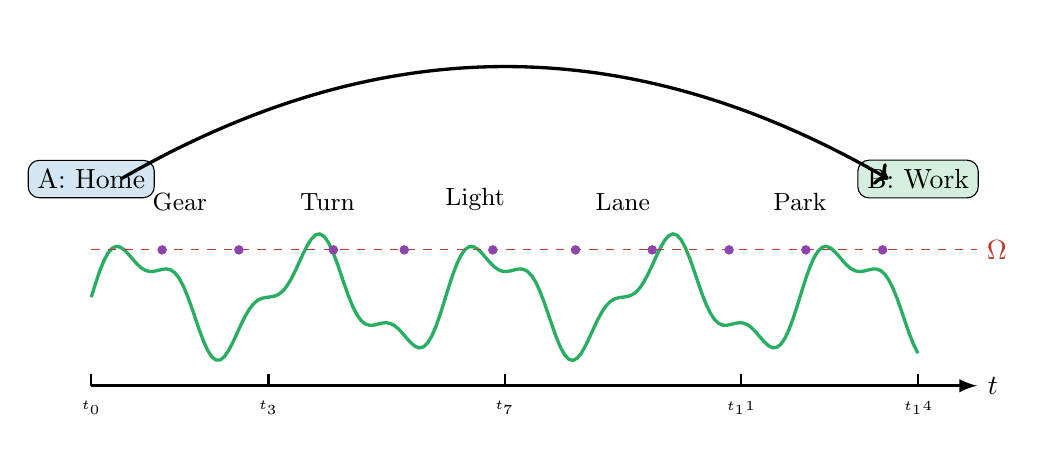
\begin{tikzpicture}[scale=0.75]
% Timeline
\draw[-latex, very thick] (0,0) -- (15,0) node[right] {$t$};

% Major phases
\foreach \x/\phase/\y in {0/Start/1, 3/Navigate/2, 7/Midpoint/1.5, 11/Navigate/2, 14/Arrive/1} {
    \draw[thick] (\x,0) -- (\x,0.2);
    \node[below] at (\x,-0.1) {\tiny $t_\x$};
}

% Coherence envelope
\draw[crrgreen, very thick, domain=0:14, samples=200]
    plot (\x, {1.5 + 0.8*sin(120*\x) + 0.3*sin(300*\x)});

% Omega threshold
\draw[dashed, goalred] (0,2.3) -- (15,2.3) node[right] {$\Omega$};

% Rupture points (where curve crosses threshold)
\foreach \x in {1.2, 2.5, 4.1, 5.3, 6.8, 8.2, 9.5, 10.8, 12.1, 13.4} {
    \filldraw[matchpurple] (\x,2.3) circle (2pt);
}

% Labels
\node[above, font=\small] at (1.5,2.8) {Gear};
\node[above, font=\small] at (4,2.8) {Turn};
\node[above, font=\small] at (6.5,2.8) {Light};
\node[above, font=\small] at (9,2.8) {Lane};
\node[above, font=\small] at (12,2.8) {Park};

% Locations
\node[draw, fill=fepblue!20, rounded corners] at (0,3.5) {A: Home};
\node[draw, fill=crrgreen!20, rounded corners] at (14,3.5) {B: Work};

% Journey arc
\draw[very thick, ->] (0.5,3.5) to[out=30, in=150] (13.5,3.5);
\end{tikzpicture}
\caption{The complete journey from A to B shown as oscillating coherence punctuated by rupture events. Each peak crossing $\Omega$ represents a micro-goal completion (gear change, turn, traffic response, etc.).}
\label{fig:journey}
\end{figure}

\subsection{Mathematical Summary of Journey}

\begin{fepbox}{Journey in FEP: Hierarchical Policy Selection}{}
The complete journey is a hierarchical policy:
\begin{equation}
\pi_{\text{journey}} = \{\pi_{\text{nav}}, \pi_{\text{vehicle}}, \pi_{\text{hazard}}\}
\end{equation}

Total expected free energy:
\begin{equation}
G(\pi_{\text{journey}}) = \sum_{k=1}^{N} \gamma^k \cdot G(\pi_k)
\end{equation}
where $\gamma < 1$ is temporal discounting and $N$ is number of sub-goals.

\textbf{Success criterion}: Arrive at B with:
\begin{equation}
D_{KL}[q(\text{location}) \| \delta_B] < \epsilon
\end{equation}
(Belief about location concentrated at B)
\end{fepbox}

\begin{crrbox}{Journey in CRR: Nested Cycle Cascade}{}
The journey consists of $N$ nested CRR cycles:
\begin{equation}
\text{Journey} = \bigcup_{k=1}^{N} \text{CRR}_k = \bigcup_{k=1}^{N} (C_k \to \Omega \to R_k)
\end{equation}

Total information processed:
\begin{equation}
I_{\text{total}} = \sum_{k=1}^{N} C_k(t^*_k) \approx N \times 16 \text{ nats}
\end{equation}

For a 20-minute journey with $\sim$100 micro-goals:
\begin{equation}
I_{\text{total}} \approx 100 \times 16 = 1600 \text{ nats} \approx 2300 \text{ bits}
\end{equation}

\textbf{Rate}: $\frac{2300 \text{ bits}}{1200 \text{ s}} \approx 2 \text{ bits/s}$ conscious processing (matches cognitive bandwidth estimates!)
\end{crrbox}

%=============================================================================
\section{The Unified Picture}
%=============================================================================

\begin{figure}[H]
\centering
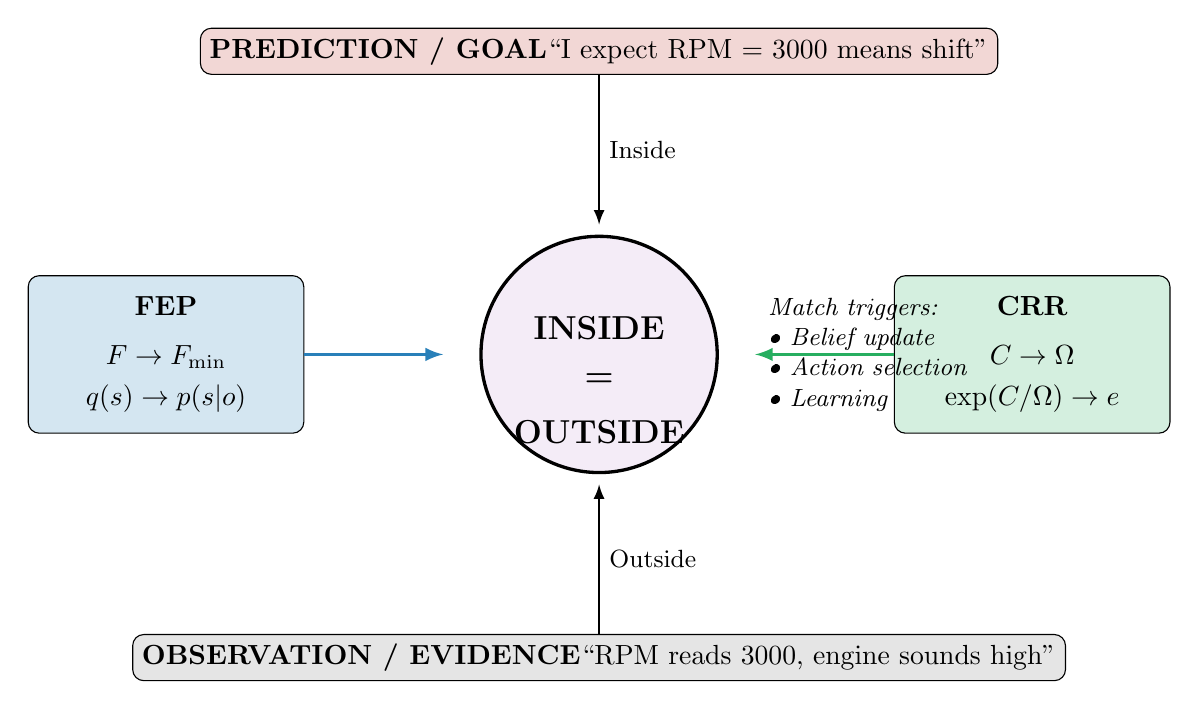
\begin{tikzpicture}[scale=1.1]
% Central diagram
\node[draw, very thick, circle, minimum size=30mm, fill=matchpurple!10] (center) at (0,0) {};
\node[font=\large\bfseries] at (0,0.3) {INSIDE};
\node[font=\large\bfseries] at (0,-0.3) {=};
\node[font=\large\bfseries] at (0,-0.9) {OUTSIDE};

% FEP side
\node[draw, rounded corners, fill=fepblue!20, minimum width=35mm, minimum height=20mm, align=center] (fep) at (-5,0) {
\textbf{FEP}\\[2mm]
$F \to F_{\min}$\\[1mm]
$q(s) \to p(s|o)$
};

% CRR side
\node[draw, rounded corners, fill=crrgreen!20, minimum width=35mm, minimum height=20mm, align=center] (crr) at (5,0) {
\textbf{CRR}\\[2mm]
$C \to \Omega$\\[1mm]
$\exp(C/\Omega) \to e$
};

% Arrows
\draw[-latex, very thick, fepblue] (fep) -- (-1.8,0);
\draw[-latex, very thick, crrgreen] (crr) -- (1.8,0);

% Top: Prediction
\node[draw, rounded corners, fill=goalred!20, minimum width=50mm] (pred) at (0,3.5) {
\textbf{PREDICTION / GOAL}\\
``I expect RPM = 3000 means shift''
};

% Bottom: Observation
\node[draw, rounded corners, fill=gray!20, minimum width=50mm] (obs) at (0,-3.5) {
\textbf{OBSERVATION / EVIDENCE}\\
``RPM reads 3000, engine sounds high''
};

% Vertical arrows
\draw[-latex, thick] (pred) -- (0,1.5) node[midway, right, font=\small] {Inside};
\draw[-latex, thick] (obs) -- (0,-1.5) node[midway, right, font=\small] {Outside};

% Match annotation
\node[right=5mm of center, font=\small\itshape, text width=30mm] {
Match triggers:\\
\textbullet\ Belief update\\
\textbullet\ Action selection\\
\textbullet\ Learning
};
\end{tikzpicture}
\caption{The unified picture: Both FEP ($F \to F_{\min}$) and CRR ($C \to \Omega$) describe the same phenomenon---the moment when internal predictions align with external observations, triggering state transitions.}
\label{fig:unified}
\end{figure}

\subsection{Why 16 Nats is the Universal Threshold}

\begin{matchbox}{The Information-Theoretic Interpretation}{}
$\Omega \approx 16$ nats $\approx 23$ bits represents:

\begin{enumerate}
    \item \textbf{Goal specification precision}: To specify a goal (``shift gear'', ``stop at light'') requires $\sim$23 bits to distinguish from $2^{23} \approx 8$ million alternatives.

    \item \textbf{Evidence sufficiency}: To confirm a goal is achieved requires accumulating $\sim$23 bits of sensory evidence across multiple channels.

    \item \textbf{Error correction capacity}: Biological systems can reliably correct errors up to $\sim 2^{23}$ states before requiring reorganization.

    \item \textbf{Thermodynamic bound}: At body temperature, $16 \times k_B T \approx 40$ kJ/mol---the typical activation barrier for molecular conformational changes.
\end{enumerate}

The convergence of cognitive, biological, and thermodynamic constraints on this value suggests it is a \textbf{fundamental constant of adaptive systems}.
\end{matchbox}

%=============================================================================
\section{Outcome-Dependent Regeneration}
%=============================================================================

\begin{figure}[H]
\centering
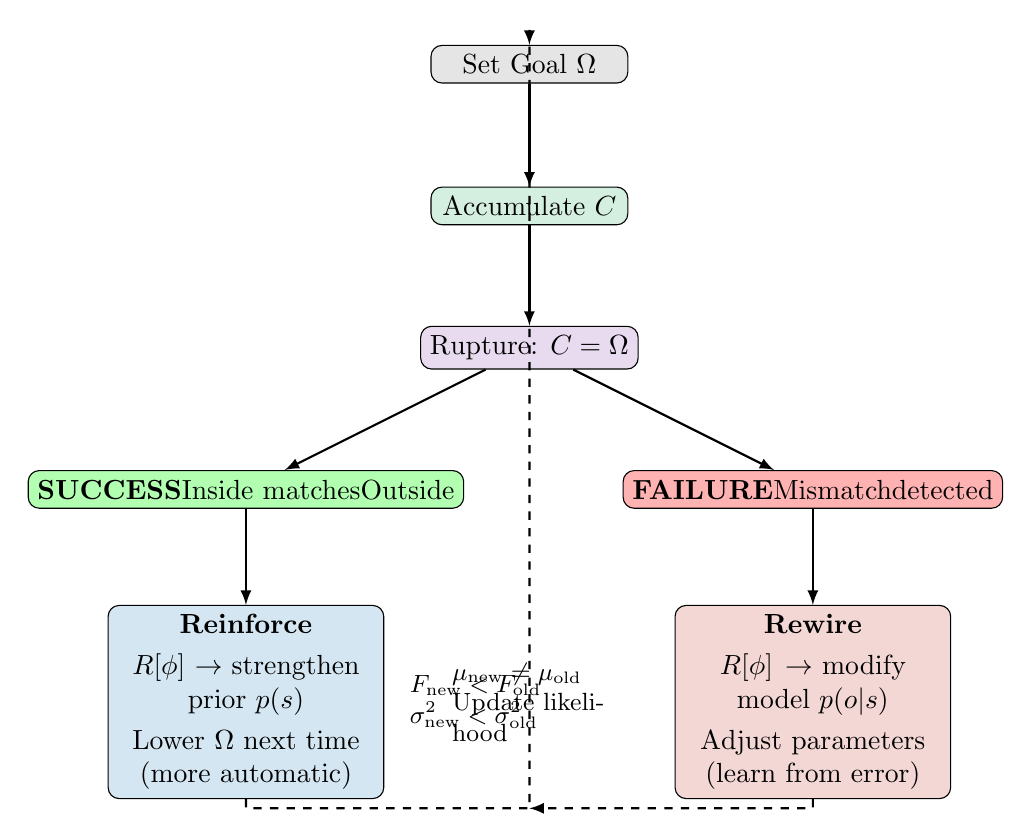
\begin{tikzpicture}[scale=0.9]
% Main flow
\node[draw, rounded corners, fill=gray!20, minimum width=25mm] (goal) at (0,4) {Set Goal $\Omega$};
\node[draw, rounded corners, fill=crrgreen!20, minimum width=25mm] (accum) at (0,2) {Accumulate $C$};
\node[draw, rounded corners, fill=matchpurple!20, minimum width=25mm] (rupture) at (0,0) {Rupture: $C = \Omega$};

\draw[-latex, thick] (goal) -- (accum);
\draw[-latex, thick] (accum) -- (rupture);

% Branch
\node[draw, rounded corners, fill=green!30, minimum width=30mm] (success) at (-4,-2) {\textbf{SUCCESS}\\Inside matches\\Outside};
\node[draw, rounded corners, fill=red!30, minimum width=30mm] (fail) at (4,-2) {\textbf{FAILURE}\\Mismatch\\detected};

\draw[-latex, thick] (rupture) -- (-2,-1) -- (success);
\draw[-latex, thick] (rupture) -- (2,-1) -- (fail);

% Outcomes
\node[draw, rounded corners, fill=fepblue!20, minimum width=35mm, text width=32mm, align=center] (reinforce) at (-4,-5) {
\textbf{Reinforce}\\[1mm]
$R[\phi] \to$ strengthen\\
prior $p(s)$\\[1mm]
Lower $\Omega$ next time\\
(more automatic)
};

\node[draw, rounded corners, fill=goalred!20, minimum width=35mm, text width=32mm, align=center] (rewire) at (4,-5) {
\textbf{Rewire}\\[1mm]
$R[\phi] \to$ modify\\
model $p(o|s)$\\[1mm]
Adjust parameters\\
(learn from error)
};

\draw[-latex, thick] (success) -- (reinforce);
\draw[-latex, thick] (fail) -- (rewire);

% Return arrows
\draw[-latex, thick, dashed] (reinforce.south) -- (-4,-6.5) -- (0,-6.5) -- (0,4.5) -- (goal.north);
\draw[-latex, thick, dashed] (rewire.south) -- (4,-6.5) -- (0,-6.5);

% Mathematical annotations
\node[right=2mm of reinforce, font=\small, text width=25mm] {
$F_{\text{new}} < F_{\text{old}}$\\
$\sigma^2_{\text{new}} < \sigma^2_{\text{old}}$
};

\node[left=2mm of rewire, font=\small, text width=25mm] {
$\mu_{\text{new}} \neq \mu_{\text{old}}$\\
Update likelihood
};
\end{tikzpicture}
\caption{The bifurcation at rupture: success leads to reinforcement (tighter priors), failure leads to rewiring (updated likelihood). Both paths use the regeneration operator $R[\phi]$ but with different effects on the generative model.}
\label{fig:bifurcation}
\end{figure}

\begin{fepbox}{Success: Precision Increase}{}
When prediction matches observation:
\begin{equation}
\Pi_{\text{new}} = \Pi_{\text{old}} + \alpha \cdot \Pi_{\text{old}} = (1 + \alpha) \Pi_{\text{old}}
\end{equation}
where $\Pi$ is precision (inverse variance) and $\alpha > 0$ is learning rate.

\textbf{Effect}: The same action becomes more automatic, requiring less conscious monitoring.
\end{fepbox}

\begin{crrbox}{Success: Lower Effective $\Omega$}{}
Successful pattern completion reduces the threshold for future recognition:
\begin{equation}
\Omega_{\text{new}} = \Omega_{\text{old}} - \beta \cdot \ln(1 + n_{\text{success}})
\end{equation}
where $n_{\text{success}}$ counts successful completions.

\textbf{Effect}: Expert drivers shift gears with minimal coherence accumulation---the pattern is automatized.
\end{crrbox}

\begin{fepbox}{Failure: Likelihood Update}{}
When prediction fails:
\begin{equation}
p_{\text{new}}(o|s) \propto p_{\text{old}}(o|s) \cdot \exp\left(-\frac{\varepsilon^2}{2\sigma^2}\right)
\end{equation}
where $\varepsilon = o_{\text{actual}} - o_{\text{predicted}}$ is prediction error.

\textbf{Effect}: The model of how states generate observations is updated to reduce future errors.
\end{fepbox}

\begin{crrbox}{Failure: Regeneration as Contrast}{}
The regeneration operator weights historical states, but now as \emph{what to change}:
\begin{equation}
R_{\text{contrast}}[\phi] = \int \phi(\tau) \cdot e \cdot (1 - \text{similarity}(\tau, t^*)) \cdot \Theta(t-\tau) \, d\tau
\end{equation}

States most similar to the failed attempt get downweighted; dissimilar states (potential alternatives) get upweighted.
\end{crrbox}

%=============================================================================
\section{Conclusion: CRR as the Grammar of Active Inference}
%=============================================================================

We have demonstrated that the CRR framework provides the \textbf{dynamical grammar} underlying active inference:

\begin{enumerate}
    \item \textbf{Coherence $C(t)$} corresponds to accumulated evidence / negative free energy
    \item \textbf{Threshold $\Omega$} corresponds to goal precision / prior certainty
    \item \textbf{Rupture $C = \Omega$} corresponds to the inside-outside match / free energy minimum
    \item \textbf{Regeneration $R[\phi]$} corresponds to posterior update / policy selection
\end{enumerate}

The universal threshold $\Omega \approx 16$ nats represents the information capacity required for:
\begin{itemize}
    \item Specifying a goal with sufficient precision
    \item Accumulating evidence sufficient for confident action
    \item Maintaining error-correction in biological computation
\end{itemize}

A driving journey from A to B consists of $\sim$100 nested CRR cycles, each following the same grammar: accumulate coherence toward a goal, rupture when evidence matches expectation, regenerate to either reinforce success or rewire after failure. This elegant recursive structure scales from millisecond motor adjustments to hour-long navigation plans, always with the same fundamental threshold of $\sim$16 nats marking the moment when inside meets outside.

\vspace{5mm}
\begin{center}
\fbox{\parbox{0.8\textwidth}{\centering
\textbf{The Central Equation}\\[3mm]
$\displaystyle \underbrace{C(t^*) = \Omega}_{\text{CRR: Rupture}} \quad \Longleftrightarrow \quad \underbrace{F(q^*) = F_{\min}}_{\text{FEP: Equilibrium}} \quad \Longleftrightarrow \quad \underbrace{\text{Inside} = \text{Outside}}_{\text{Phenomenology: Recognition}}$
}}
\end{center}

\end{document}
